\begin{figure}[p]\centering
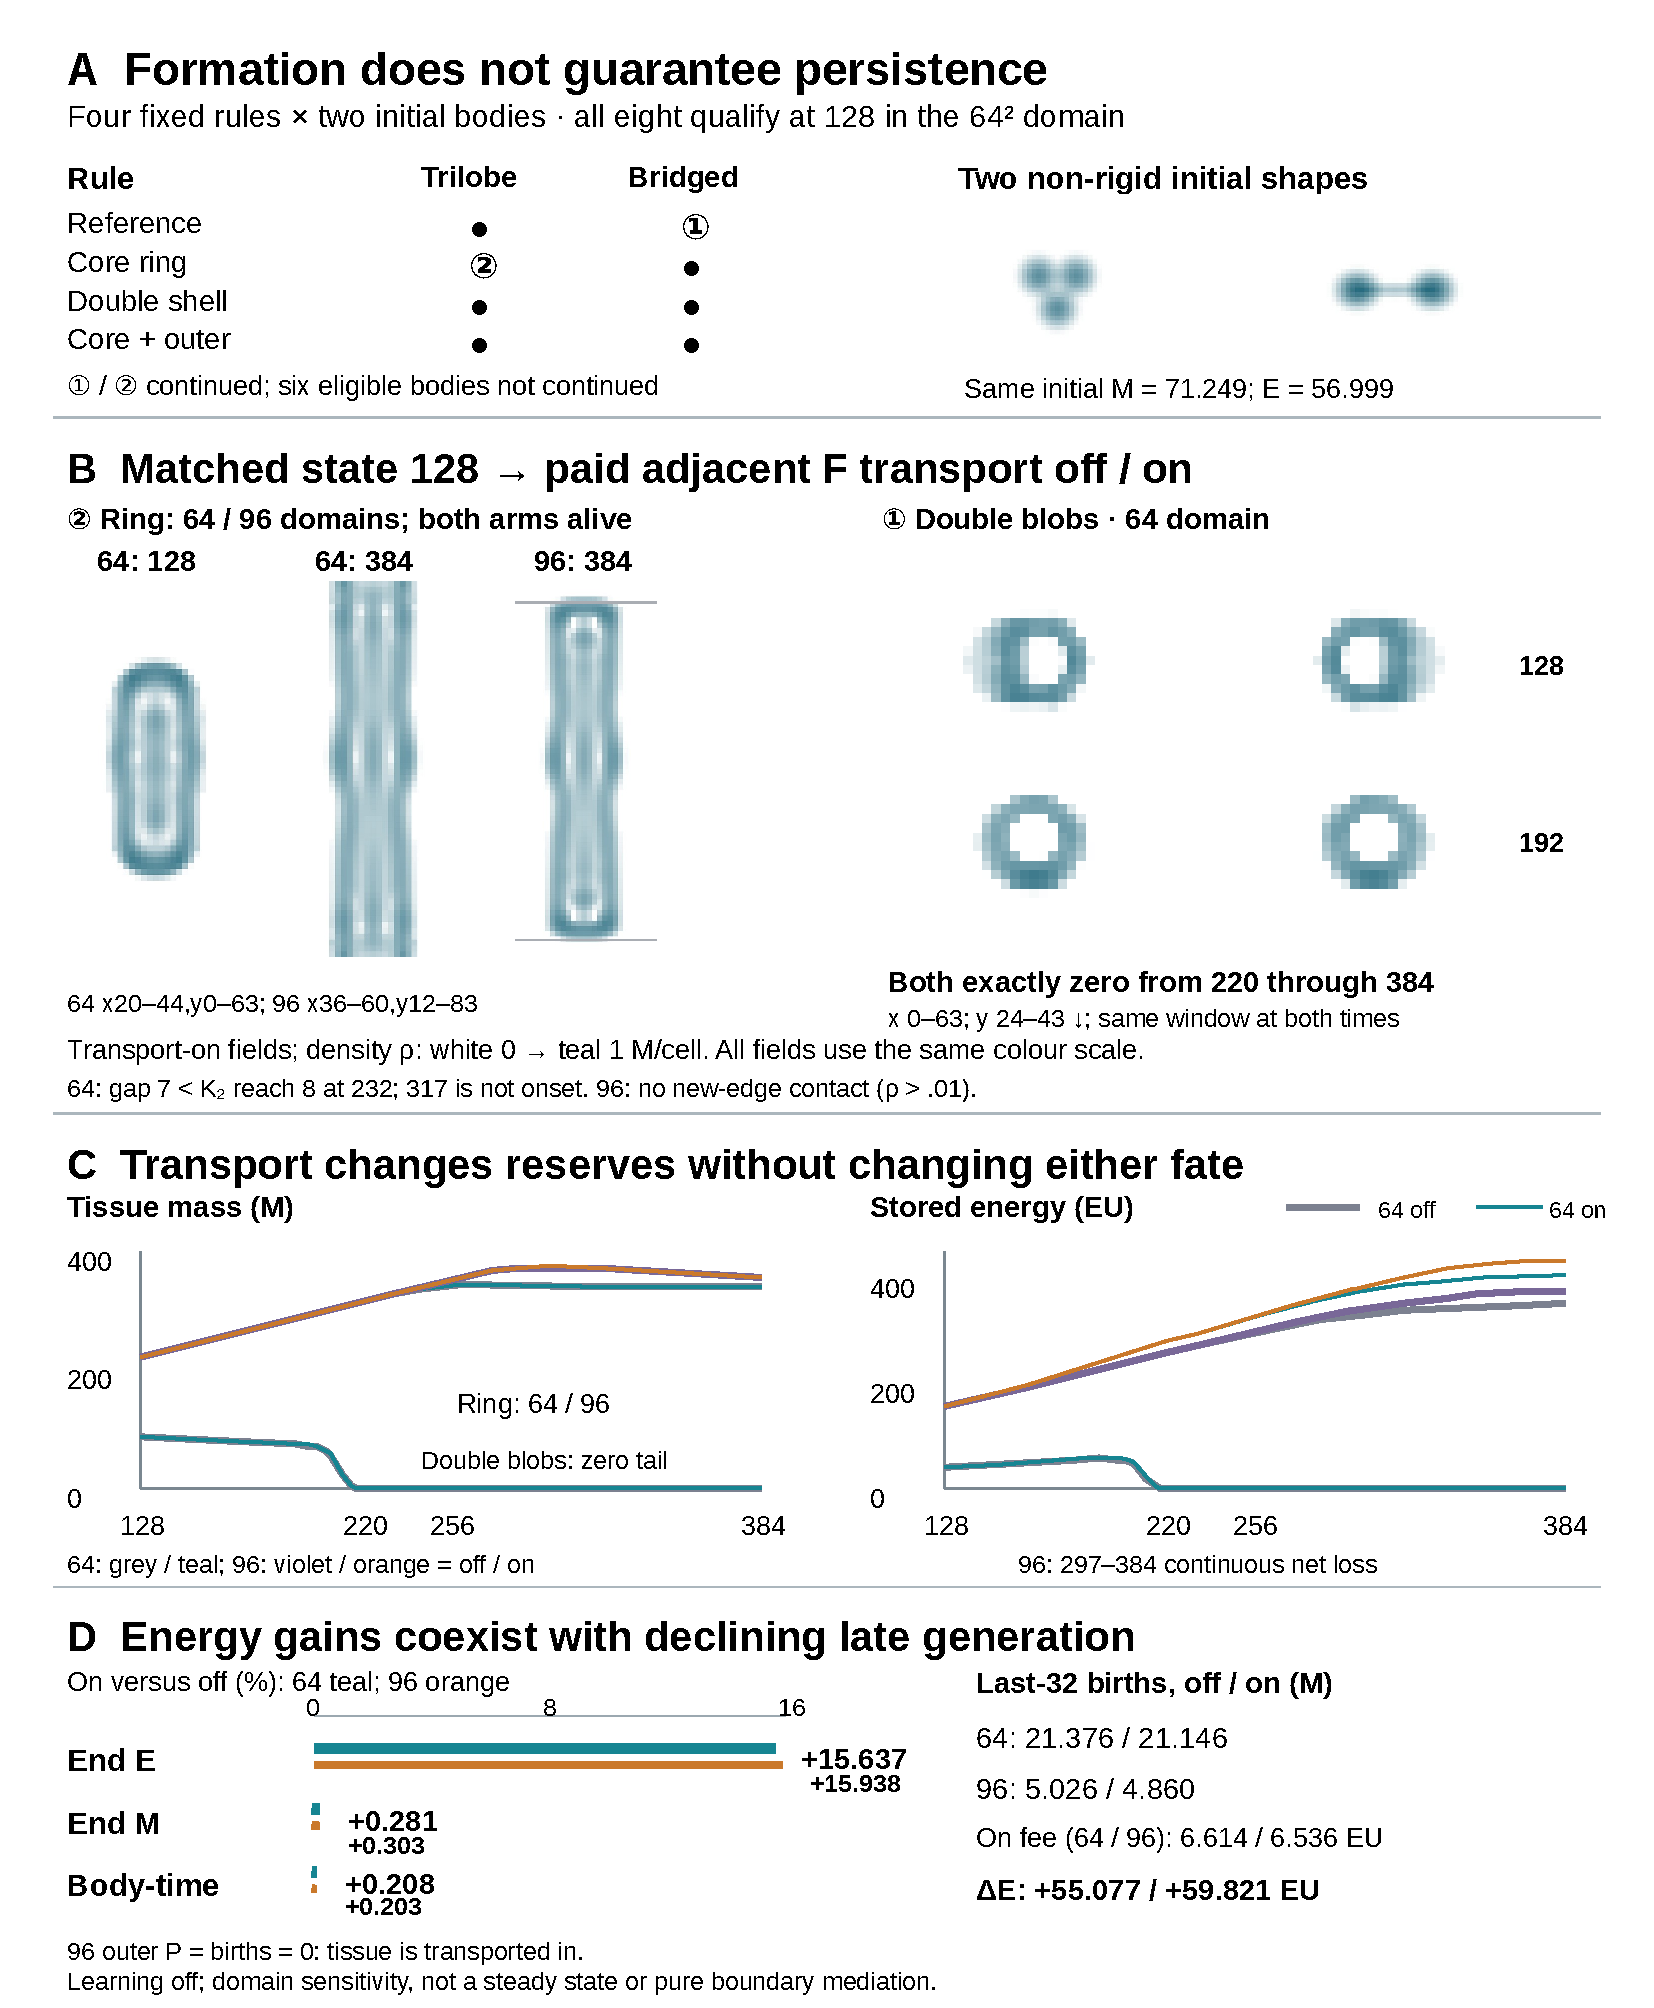
\includegraphics[width=\linewidth,height=.76\textheight,keepaspectratio]{figures/main/formation/regenerative_morphology_transport.pdf}
\caption{\textbf{Formation, persistence and the energetic value of fuel transport differ.} \textbf{a,} Eight rule/initial-field combinations qualify at 128; six are uncontinued. \textbf{b,} True density fields preserve original coordinates and a common scale. Both separated-body futures become extinct; the ring persists in both domains. \textbf{c,} Complete mass and energy paths retain zero tails and late loss. \textbf{d,} Within-domain on-minus-off effects show much larger energy than tissue/body-time gains. Outer tissue in the larger domain arrives by transport without local birth in this comparison. The embedding changes the whole domain condition, not an isolated boundary mediator. These selected dependent paths do not establish learning or stable maintenance.}
\label{fig:formation-persistence}\end{figure}
